Om het uiteindelijke oordeel te vellen of filteren al dan niet een verbeterende factor kan zijn binnen het project, doet het verslag nog een laatste vergelijking. Namelijk kijken naar het verschil in juist gedetecteerde afbeeldingen per gebruikte methode alsook zonder het gebruik van een filter.

\begin{figure}[h!]
  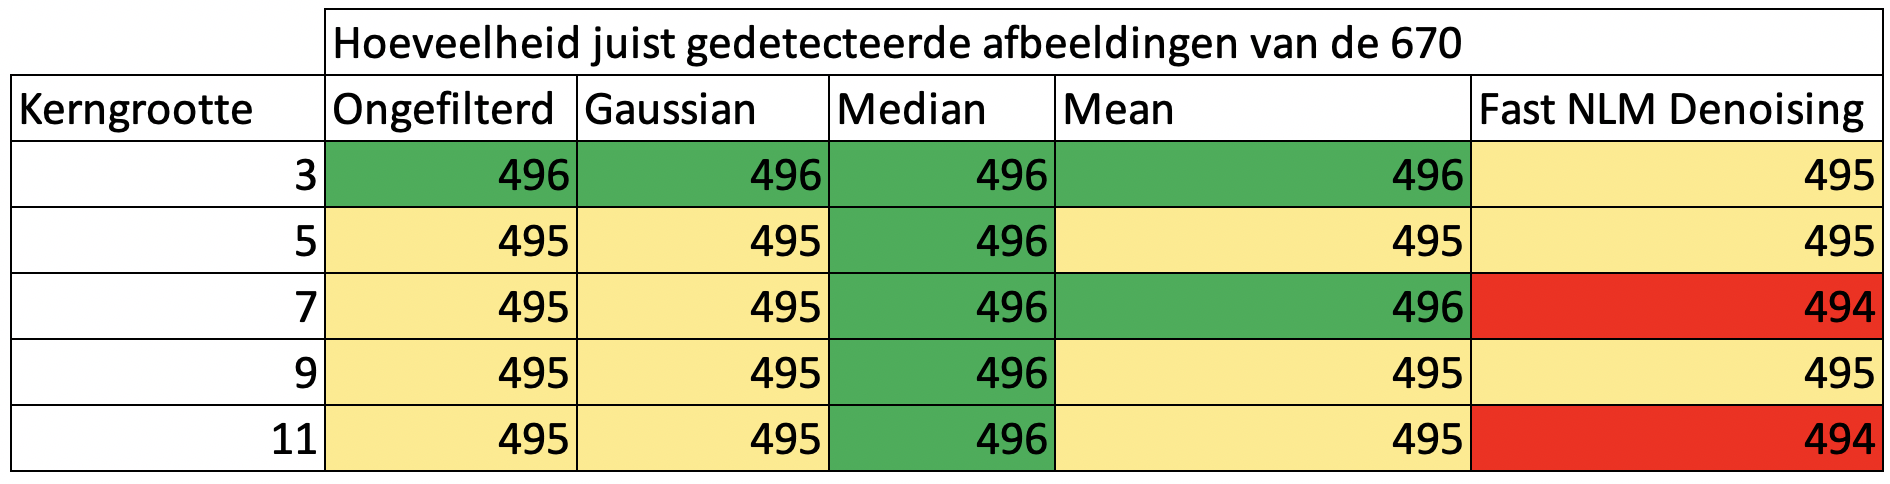
\includegraphics[width=\linewidth]{img/filternofilter}
  \caption{Aantal juist gedetecteerde foto's van de 670, gegeven de gebruikte filter.}
  \label{fig:filternofilter}
\end{figure}

Ook hier zijn de waarden nagenoeg gelijk, van de 670 afbeelding worden er bij elke toegepaste filter en gebruikte kerngrootte gemiddeld 495 correct gedetecteerd. Dit wijkt slechts af met maximaal één. Hieruit volgt alweer dat een filter toepassen nagenoeg geen effect heeft op het detecteren van de kleuren.